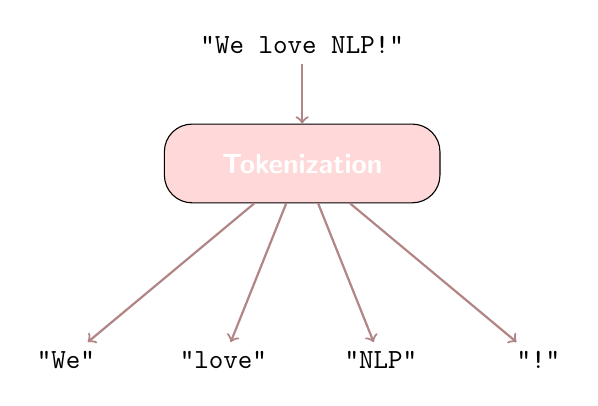
\begin{tikzpicture}[every node/.style={font=\sffamily}, node distance=1.2cm and 2cm, align=center]
        % Sentence input
        \node (sentence) at (0, 4) {\texttt{"We love NLP!"}};

        % Tokenization box
        \node[draw, rounded corners=10pt, fill=pink!60, text=white, minimum width=3.5cm, minimum height=1cm] (tokenization) at (0, 2.5) {\textbf{Tokenization}};

        % Tokens on a straight line
        \node (we) at (-3, 0) {\texttt{"We"}};
        \node (love) at (-1, 0) {\texttt{"love"}};
        \node (nlp) at (1, 0) {\texttt{"NLP"}};
        \node (punct) at (3, 0) {\texttt{"!"}};

        % Arrows
        \draw[->, thick, pink!70!black] (sentence) -- (tokenization);
        \draw[->, thick, pink!70!black] (tokenization) -- (we);
        \draw[->, thick, pink!70!black] (tokenization) -- (love);
        \draw[->, thick, pink!70!black] (tokenization) -- (nlp);
        \draw[->, thick, pink!70!black] (tokenization) -- (punct);
\end{tikzpicture}